\chapter{A tabela periódica: um primeiro olhar}\label{ch:g9:periodic-table-first-look}

Na parede de quase toda sala de química está pendurado o mesmo quadro:
118 casas, cada uma com um símbolo e um número, organizadas em linhas e
colunas com uma forma estranha --- torres altas dos lados, um rebaixo no
meio, duas linhas soltas embaixo. Quando ele foi desenhado pela primeira
vez, em 1869, tinha umas sessenta casas e várias vazias. O seu autor
teve a ousadia de descrever os elementos que um dia preencheriam as
lacunas --- e acertou.

\begin{recall}
Um \omterm{def:g9:inside-the-atom:element}{elemento químico} é o conjunto dos \omterm{def:g7:atoms-and-molecules:atom}{átomos} com o mesmo \omterm{def:g9:inside-the-atom:atomic-number}{número atômico}
$Z$, o número de \omterm{def:g9:inside-the-atom:proton}{prótons} do \omterm{def:g9:inside-the-atom:nucleus}{núcleo} (\cref{ch:g9:inside-the-atom}). Cada
elemento tem um símbolo, uma letra maiúscula às vezes seguida de uma
minúscula (\cref{ch:g7:atoms-and-molecules}). Os \omterm{def:g9:periodic-table-first-look:metal}{metais}, como o ferro, o
zinco e o alumínio, dão \omterm{def:g9:ions:ion}{íons} positivos (\cref{ch:g9:ions}).
\end{recall}

\section{Uma tabela dos elementos}

\begin{definition}[Tabela periódica]\label{def:g9:periodic-table-first-look:periodic-table}
A \emph{tabela periódica}\index{tabela periodica@tabela periódica} lista todos os
\omterm{def:g9:inside-the-atom:element}{elementos químicos} em ordem crescente de \omterm{def:g9:inside-the-atom:atomic-number}{número atômico}, de $Z = 1$ a
$Z = 118$, organizados em linhas de modo que os elementos com
propriedades parecidas fiquem na mesma coluna.
\end{definition}

\begin{definition}[Período e grupo]\label{def:g9:periodic-table-first-look:period}
Uma linha da \omterm{def:g9:periodic-table-first-look:periodic-table}{tabela periódica} é um \emph{período}\index{periodo@período}; há
sete. Uma coluna é um \emph{grupo}\index{grupo}; há dezoito, numerados
de 1 a 18 da esquerda para a direita. As duas linhas impressas abaixo da
tabela pertencem aos períodos 6 e 7; elas só ficam separadas para manter
a tabela estreita.
\end{definition}

\begin{omfigure}
\omperiodictable[colour=metals, legend=true, cell=0.86cm]

{\small A \omterm{def:g9:periodic-table-first-look:periodic-table}{tabela periódica}. Cada casa dá o \omterm{def:g9:inside-the-atom:atomic-number}{número atômico} e o símbolo.
Cores: \omterm{def:g9:periodic-table-first-look:metal}{metais}, metaloides (elementos entre os \omterm{def:g9:periodic-table-first-look:metal}{metais} e os \omterm{def:g9:periodic-table-first-look:metal}{não metais}) e
\omterm{def:g9:periodic-table-first-look:metal}{não metais}, na classificação usual.}
\end{omfigure}

\begin{method}[Ler a tabela periódica]\label{met:g9:periodic-table-first-look:read}
Para localizar um elemento:
\begin{enumerate}
  \item encontre a casa dele pelo símbolo ou pelo \omterm{def:g9:inside-the-atom:atomic-number}{número atômico};
  \item a linha dá o \omterm{def:g9:periodic-table-first-look:period}{período}, a coluna dá o grupo;
  \item a cor diz se ele é um \omterm{def:g9:periodic-table-first-look:metal}{metal} ou um \omterm{def:g9:periodic-table-first-look:metal}{não metal}.
\end{enumerate}
Sódio, \ce{Na}, $Z = 11$: \omterm{def:g9:periodic-table-first-look:period}{período} 3, \omterm{def:g9:periodic-table-first-look:period}{grupo} 1, um \omterm{def:g9:periodic-table-first-look:metal}{metal}. Cloro,
\ce{Cl}, $Z = 17$: \omterm{def:g9:periodic-table-first-look:period}{período} 3, \omterm{def:g9:periodic-table-first-look:period}{grupo} 17, um \omterm{def:g9:periodic-table-first-look:metal}{não metal}.
\end{method}

\section{Metais e não metais}

\begin{definition}[Metal e não metal]\label{def:g9:periodic-table-first-look:metal}
Um \emph{metal}\index{metal} é um elemento que, como \omterm{def:g6:pure-substances-and-mixtures:pure-substance}{substância pura}, é
brilhante quando acabou de ser cortado, conduz bem a eletricidade e o
calor, pode ser dobrado ou moldado a marteladas, e forma \omterm{def:g9:ions:ion}{íons} positivos.
Um \emph{não metal}\index{nao metal@não metal} não tem essas propriedades: muitos
são gases (o oxigênio, o nitrogênio, o cloro), os sólidos são opacos e
quebradiços (o enxofre, o carbono na forma de carvão), e eles tendem a
formar \omterm{def:g9:ions:ion}{íons} negativos ou a compartilhar \omterm{def:g9:inside-the-atom:nucleus}{elétrons} em \omterm{def:g7:atoms-and-molecules:molecule}{moléculas}.
\end{definition}

\begin{proposition}[Onde eles ficam]\label{prop:g9:periodic-table-first-look:where}
Cerca de quatro elementos em cada cinco são \omterm{def:g9:periodic-table-first-look:metal}{metais}; eles ocupam a
esquerda e o centro da tabela. Os \omterm{def:g9:periodic-table-first-look:metal}{não metais} ficam no alto, à direita,
com o hidrogênio sozinho no alto, à esquerda. Ao longo da fronteira
entre eles, alguns elementos --- boro, silício, germânio, arsênio,
antimônio, telúrio --- têm propriedades intermediárias: os metaloides.
\end{proposition}

\section{Colunas que se comportam igual}

\begin{proposition}[Os elementos de um grupo se comportam igual]\label{prop:g9:periodic-table-first-look:alike}
Os elementos de um mesmo grupo reagem de modos parecidos e formam
compostos parecidos. O lítio, o sódio e o potássio, no alto do \omterm{def:g9:periodic-table-first-look:period}{grupo} 1,
são \omterm{def:g9:periodic-table-first-look:metal}{metais} moles que reagem com a água, liberando hidrogênio; a reação é
mais violenta à medida que se desce no grupo. O flúor, o cloro, o bromo
e o iodo, no \omterm{def:g9:periodic-table-first-look:period}{grupo} 17, são \omterm{def:g9:periodic-table-first-look:metal}{não metais} coloridos que reagem com os \omterm{def:g9:periodic-table-first-look:metal}{metais}
formando sais. O hélio, o neônio, o argônio e os outros elementos do
\omterm{def:g9:periodic-table-first-look:period}{grupo} 18 quase não reagem com nada.
\end{proposition}

\begin{inthelab}[Lítio, sódio e potássio na água]
Atrás de uma tela de proteção, o professor joga um pedaço de lítio do
tamanho de um grão de arroz numa bacia grande com água: ele borbulha de
leve. Um pedaço de sódio do mesmo tamanho dispara pela superfície,
derretendo numa bolinha prateada. O potássio pega fogo na hora, com uma
chama lilás. Os três liberam hidrogênio e deixam uma \omterm{def:g9:acids-bases-ph:acidic}{solução básica}.
\end{inthelab}

\begin{safety}{\ghs[0.82cm]{GHS02}\ghs[0.82cm]{GHS05}}
% ledger: ghs:Na
Sódio: em contato com a água, libera gases inflamáveis que podem
pegar fogo (GHS02); provoca queimaduras graves (GHS05). Ele é guardado
sob óleo e manuseado só pelo professor, com uma pinça, em pedaços
minúsculos.
\end{safety}

\section{A ideia de Mendeleiev}

\begin{history}[As lacunas de Mendeleiev, 1869--1886]
Em 1869, Dmitri Mendeleiev organizou os elementos então conhecidos em
ordem crescente de peso atômico --- a massa dos seus \omterm{def:g7:atoms-and-molecules:atom}{átomos} comparada
com a do hidrogênio --- e colocou lado a lado os que tinham propriedades
parecidas. Onde o padrão exigia, ele deixou lacunas para elementos que
ninguém tinha encontrado ainda, e em 1871 descreveu as propriedades
deles: abaixo do silício, um ``eka-silício'' cujo peso atômico seria
cerca de 72. Em 1886, o químico Clemens Winkler descobriu o germânio num
\omterm{def:g5:raw-materials-and-recycling:raw-material}{minério} de prata, mediu o seu peso atômico, 72.3, e viu que era o
elemento que faltava. O gálio (1875) e o escândio (1879) também
preencheram lacunas deixadas por Mendeleiev.
\end{history}

\begin{omfigure}
\begin{minipage}[b]{0.32\linewidth}\centering
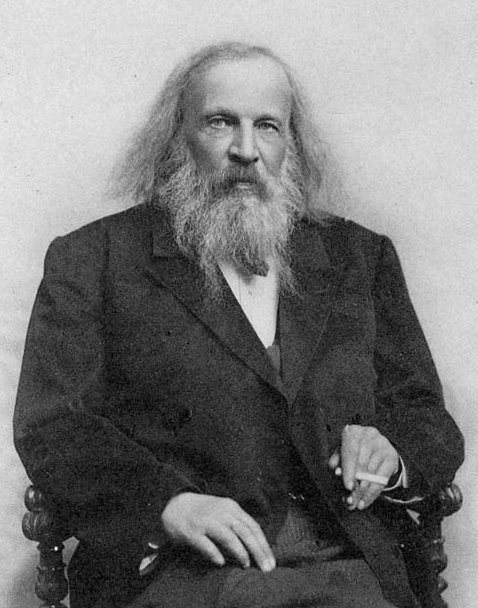
\includegraphics[width=\linewidth]{images/book1/mendeleev.jpg}

{\small Dmitri Mendeleiev (1834--1907).}
\end{minipage}\hfill
\begin{minipage}[b]{0.6\linewidth}\centering
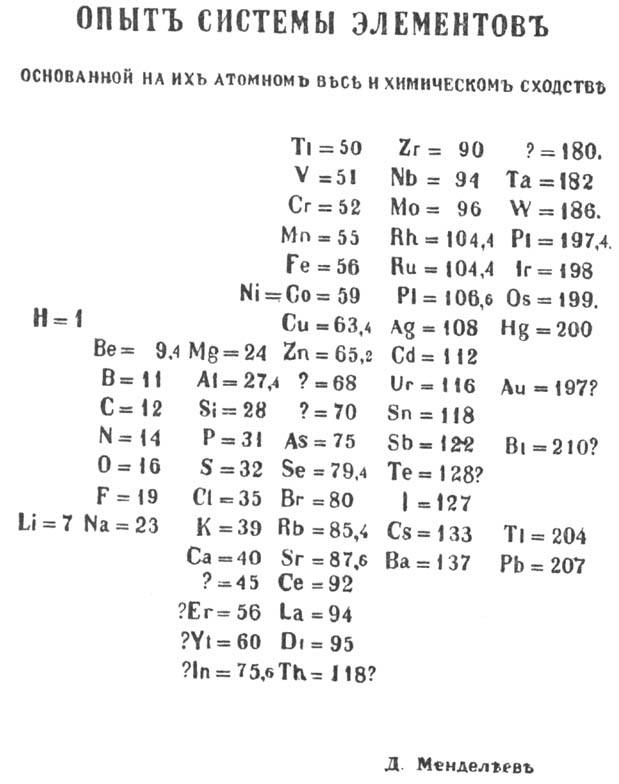
\includegraphics[width=0.85\linewidth]{images/book1/mendeleev-1869.jpg}

{\small A tabela de Mendeleiev de 1869, em russo. Ao lado de Si $= 28$ e
Al $= 27.4$, as lacunas ``? $= 70$'' e ``? $= 68$'' esperam o germânio
e o gálio.}
\end{minipage}
\end{omfigure}

\begin{remark}[Ordem por número atômico]\label{rem:g9:periodic-table-first-look:order}
Mendeleiev ordenou os elementos pelo peso atômico, e teve de trocar de
lugar alguns pares, como o telúrio e o iodo, para manter as famílias
juntas. Hoje a tabela é ordenada pelo \omterm{def:g9:inside-the-atom:atomic-number}{número atômico}, descoberto mais
tarde, e as trocas não são mais necessárias.
\end{remark}

\section{Exercícios}

\begin{exercise}[$\star$]\label{exo:g9:periodic-table-first-look:1}
Em que ordem os elementos são colocados na \omterm{def:g9:periodic-table-first-look:periodic-table}{tabela periódica}?
\end{exercise}

\begin{exercise}[$\star$]\label{exo:g9:periodic-table-first-look:2}
Dê o \omterm{def:g9:periodic-table-first-look:period}{período} e o grupo do carbono ($Z = 6$), do magnésio ($Z = 12$) e
do argônio ($Z = 18$).
\end{exercise}

\begin{exercise}[$\star$]\label{exo:g9:periodic-table-first-look:3}
\omterm{def:g9:periodic-table-first-look:metal}{Metal} ou \omterm{def:g9:periodic-table-first-look:metal}{não metal}: ferro, enxofre, cobre, oxigênio, alumínio, cloro?
\end{exercise}

\begin{exercise}[$\star$]\label{exo:g9:periodic-table-first-look:4}
Que elemento fica logo abaixo do sódio na tabela? E logo abaixo do
cloro?
\end{exercise}

\begin{exercise}[$\star\star$]\label{exo:g9:periodic-table-first-look:5}
Usando a tabela, dê o nome do elemento do \omterm{def:g9:periodic-table-first-look:period}{período} 4 e do \omterm{def:g9:periodic-table-first-look:period}{grupo} 2, e o do
elemento do \omterm{def:g9:periodic-table-first-look:period}{período} 2 e do \omterm{def:g9:periodic-table-first-look:period}{grupo} 15.
\end{exercise}

\begin{exercise}[$\star\star$]\label{exo:g9:periodic-table-first-look:6}
Por que se pode esperar que o potássio reaja com a água, como o sódio?
\end{exercise}

\begin{exercise}[$\star\star$]\label{exo:g9:periodic-table-first-look:7}
Um elemento brilhante conduz a eletricidade e forma o \omterm{def:g9:ions:ion}{íon} \ce{X^{2+}}.
Ele é um \omterm{def:g9:periodic-table-first-look:metal}{metal} ou um \omterm{def:g9:periodic-table-first-look:metal}{não metal}? Explique.
\end{exercise}

\begin{exercise}[$\star\star$]\label{exo:g9:periodic-table-first-look:8}
Por que Mendeleiev deixou lacunas na tabela dele? Por que isso era um
ponto forte da tabela, e não uma fraqueza?
\end{exercise}

\begin{exercise}[$\star\star$]\label{exo:g9:periodic-table-first-look:9}
Olhe a tabela de Mendeleiev de 1869. Que pesos atômicos ele deu para o
carbono e para o oxigênio? Que duas lacunas, marcadas com um ponto de
interrogação, aparecem ao lado do alumínio e do silício?
\end{exercise}

\begin{exercise}[$\star\star$]\label{exo:g9:periodic-table-first-look:10}
Quantos elementos há no \omterm{def:g9:periodic-table-first-look:period}{período} 2? E no \omterm{def:g9:periodic-table-first-look:period}{período} 4?
\end{exercise}

\begin{exercise}[$\star\star\star$]\label{exo:g9:periodic-table-first-look:11}
O hélio, o neônio e o argônio quase não reagem com nada. Em que grupo
eles estão? Para que eles poderiam ser usados, dada essa propriedade?
\end{exercise}

\begin{exercise}[$\star\star\star$]\label{exo:g9:periodic-table-first-look:12}
O gálio, abaixo do alumínio, foi descoberto em 1875. Mendeleiev tinha
previsto para ele um peso atômico próximo da média dos seus vizinhos, o
alumínio (27.0) e o índio (114.8). Calcule essa média. (Gálio: 69.7.)
\end{exercise}

\section{Problema: a lacuna de Mendeleiev}

\begin{problem}[{Problema de fim de semana --- prever o peso atômico de
um elemento que falta a partir dos seus quatro vizinhos}]
\label{pb:g9:periodic-table-first-look:1}
% ledger: aw:Si, aw:Sn, aw:Ga, aw:As, aw:Ge, mend:eka-si-aw, ge:winkler-aw
Em 1871, Mendeleiev previu as propriedades do eka-silício, o elemento
que faltava abaixo do silício. Uma das suas ideias era que as
propriedades de um elemento ficam entre as dos seus vizinhos de cima e
de baixo, da esquerda e da direita. Os pesos atômicos atuais dos quatro
vizinhos da lacuna são: silício 28.1 (em cima), estanho 118.7
(embaixo), gálio 69.7 (à esquerda), arsênio 74.9 (à direita).

\medskip
\noindent\textbf{Parte I --- A lacuna.}
\begin{enumerate}
  \item Usando a \omterm{def:g9:periodic-table-first-look:periodic-table}{tabela periódica} deste capítulo, encontre o \omterm{def:g9:inside-the-atom:atomic-number}{número
        atômico}, o \omterm{def:g9:periodic-table-first-look:period}{período} e o grupo do germânio, o elemento que preenche
        a lacuna.
  \item Que elemento fica em cima dele, qual embaixo, qual à esquerda,
        qual à direita?
  \item O germânio é um \omterm{def:g9:periodic-table-first-look:metal}{metal}, um \omterm{def:g9:periodic-table-first-look:metal}{não metal} ou um metaloide?
  \item Por que Mendeleiev esperava que o elemento que faltava se
        parecesse com o silício?
\end{enumerate}

\medskip
\noindent\textbf{Parte II --- Médias.}
\begin{enumerate}[resume]
  \item Calcule a média dos pesos atômicos dos elementos de cima e de
        baixo da lacuna.
  \item Calcule a média dos pesos atômicos dos elementos da esquerda e
        da direita.
  \item Qual das duas médias está mais perto do verdadeiro peso atômico
        do germânio, 72.6? Por que isso poderia acontecer?
  \item Na tabela de 1869, Mendeleiev tinha escrito ``? $= 70$'' para
        essa lacuna. Por quanto ele errou?
\end{enumerate}

\medskip
\noindent\textbf{Parte III --- A previsão.}
\begin{enumerate}[resume]
  \item Calcule a média dos quatro vizinhos, com uma casa decimal.
  \item Em 1871, Mendeleiev previu 72; em 1886, Winkler mediu 72.3.
        Compare com a sua média.
  \item Por que a descoberta do germânio convenceu muitos químicos de que
        a tabela de Mendeleiev estava certa?
  \item Enuncie a sua previsão: o peso atômico do eka-silício a partir da
        média dos seus quatro vizinhos.
\end{enumerate}
\end{problem}
